\iffalse

    \author{EE24BTECH11029}
    \section{ph}
    \chapter{2020}
\fi

\item Let $|e_1\rangle=\myvec{1\\0\\0},|e_2\rangle=\myvec{1\\1\\0},|e_3\rangle=\myvec{1\\1\\1}$.Let $S=\cbrak{\vec{e_1},\vec{e_2},\vec{e_3}}.$Let $\vec{R}^3$ denote the three dimensional real vector space.Which one of the following is correct?
    \begin{enumerate}
        \item $S$ is an orthonormal set
        \item $S$ is a linearly dependent set
        \item $S$ is a basis for $\vec{R}^3$
        \item $\sum_{i=1}^{3}= |e_i\rangle\langle e_i|=\myvec{1&0&0\\0&1&0\\0&0&1}$
    \end{enumerate}
    \item $\vec{S_x}$ denotes the spin operator defined as $S_x=\frac{h}{2}\myvec{0&1\\1&0}.$Which one of the following is correct?
    \begin{enumerate}
        \item The eigenstates spin operator $S_x$ are $|\uparrow\rangle=\myvec{1\\0} $ and $|\downarrow\rangle_x=\myvec{0\\1}$
        \item  The eigenstates spin operator $S_x$ are $|\uparrow\rangle=\frac{1}{\sqrt{2}}\myvec{1\\-} $ and $|\downarrow\rangle_x=\frac{1}{\sqrt{2}}\myvec{1\\1}$
        \item In the spin state $\frac{1}{2}\cbrak{\frac{1}{\sqrt{3}}},$upon the measurement of $\vec{S_x},$ the probability for obtaining $|\uparrow\rangle_x$ is $\frac{2+\sqrt{3}}{4}$
        \item In the spin state $\frac{1}{2}\cbrak{\frac{1}{\sqrt{3}}},$upon the measurement of $\vec{S_x},$ the probability for obtaining $|\uparrow\rangle_x$ is $\frac{1}{4}$
    \end{enumerate}
    \item The input voltage $\brak{\vec{V}_{in}}$ to the circuit shown in the figure is $2\cos\brak{100t}V.$The output voltage $\brak{\vec{V}_{out}}$ is $2\cos\brak{100t-\frac{\pi}{2}}V.$If value of $C\brak{in\mu F}$ is
\begin{circuitikz}
    \draw[thick](-0.5,0)node[anchor=east]{$V_{in}$} -- (0,0);
    \draw (0,0.25) to[R=$R$] (3,0.25);
    \draw (0,-0.45) to[R=$R$] (3,-0.45);
    \draw (2.3,-0.45) to[C=$C$] (2.3,-1) node[ground]{};
    \draw[thick] (3,0.75) -- (3,-0.75);
    \draw[thick] (3,0.75) -- (4,0);
    \draw[thick] (3,-0.75) -- (4,0);
    \draw[thick] (4,0)node[anchor=west]{$V_{out}$} -- (5,0);
    \draw (2.3,1) to[R=$R$] (4.3,1);
    \draw[thick] (0,0.25) -- (0,-0.45);
    \draw[thick] (2.3,1) -- (2.3,0.25);
    \draw[thick] (4.3,1) -- (4.3,0);
\end{circuitikz}

    \begin{enumerate}
        \item $0.1$
        \item $1$
        \item $10$
        \item $100$
    \end{enumerate}
    \item Consider a $4$-bit counter constructed out of four flip-flops. It is formed by connecting the $J$ and $K$ inputs to logic high and feeding the $Q$ output to the clock input of the following flip-flop . The input signal to the counter is a series of square pulses and the change of state is triggered by the falling edge. At time $t=t_0$ the outputs are in logic low state $\brak{Q_0=Q_1=Q_2=Q_3=0}.$ Then at $t=t_1$, the logic state of the outputs is


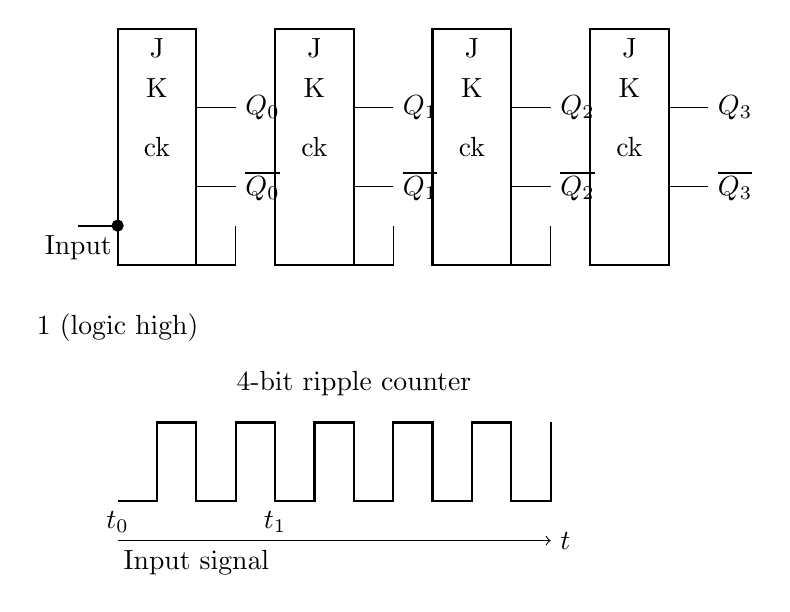
\begin{tikzpicture}
    % Flip-flops
    \foreach \i in {0, 1, 2, 3} {
        % Draw flip-flop box
        \draw[thick] (2*\i, 0) rectangle (2*\i+1, 3);
        \node at (2*\i+0.5, 2.75) {J};
        \node at (2*\i+0.5, 2.25) {K};
        \node at (2*\i+0.5, 1.5) {ck};
        
        % Q and Q' outputs
        \draw (2*\i+1, 2) -- ++(0.5, 0) node[right] {$Q_{\i}$};
        \draw (2*\i+1, 1) -- ++(0.5, 0) node[right] {$\overline{Q_{\i}}$};
    }

    % Input signal and clock
    \draw[thick] (-0.5, 0.5) -- (0, 0.5) -- (0, 2.5);
    \node[below] at (-0.5, 0.5) {Input};

    % Logic high label
    \node[below] at (0, -0.5) {1 (logic high)};
    \draw[fill] (0, 0.5) circle (2pt);
    
    % Connections between flip-flops
    \foreach \i in {1, 2, 3} {
        \draw (2*\i-1, 0.5) -- ++(0, -0.5) -- ++(0.5, 0) -- ++(0, 0.5);
    }
    
    % Label for the circuit
    \node at (3, -1.5) {4-bit ripple counter};
    
    % Input signal waveform
    \begin{scope}[shift={(0, -3)}]
        \draw[thick] (0, 0) -- (0.5, 0) -- (0.5, 1) -- (1, 1) -- (1, 0) -- (1.5, 0) -- (1.5, 1) -- (2, 1)--(2,0)--(2.5,0)--(2.5,1)--(3,1)--(3,0)--(3.5,0)--(3.5,1)--(4,1)--(4,0)--(4.5,0)--(4.5,1)--(5,1)--(5,0)--(5.5,0)--(5.5,1);
        \node[below] at (0, 0) {$t_0$};
        \node[below] at (2, 0) {$t_1$};
        \node[below] at (1, -0.5) {Input signal};
        \draw[->] (0, -0.5) -- (5.5, -0.5) node[right] {$t$};
    \end{scope}

\end{tikzpicture}
    \begin{enumerate}
        \item $Q_{0}=1,Q_{1}=0,Q_{2}=0,Q_{3}=0$
        \item $Q_{0}=0,Q_{1}=0,Q_{2}=0,Q_{3}=1$
        \item $Q_{0}=1,Q_{1}=0,Q_{2}=1,Q_{3}=0$
        \item $Q_{0}=0,Q_{1}=1,Q_{2}=1,Q_{3}=1$
    \end{enumerate}
    \item Consider the Lagrangian $L=a\brak{\frac{dx}{dy}}^2+b\brak{\frac{dy}{dt}}^2+cxy,$ where $a,b$ and $c$ are constants.If $P_x$ and $P_y$ are the momenta conjugate to the coordinates $x$ and $y$ respectively, then the Hamiltonian is
    \begin{enumerate}
        \item $\frac{P^2x}{4a}+\frac{P^2y}{4b}-cxy$
        \item $\frac{P^2x}{2a}+\frac{P^2y}{2b}-cxy$
        \item $\frac{P^2x}{2a}+\frac{P^2y}{2b}+cxy$
        \item $\frac{P^2x}{a}+\frac{P^2y}{b}+cxy$
    \end{enumerate}
    \item Which one of the following matrices does NOT represent a proper rotation in a plane?
    \begin{enumerate}
        \item $\myvec{-\sin\theta&\cos\theta\\-\cos\theta&-\sin\theta}$
        \item $\myvec{\cos\theta&\sin\theta\\-\sin\theta&\cos\theta}$
        \item $\myvec{\sin\theta&\cos\theta\\-\cos\theta&\sin\theta}$
        \item $\myvec{-\sin\theta&\cos\theta\\-\cos\theta&\sin\theta}$  
    \end{enumerate}
    \item A uniform magnetic field $\vec{B}=B_0\vec{y}$ exits in a inertial frame $K$. A perfect conducting sphere moves with a constant velocity $\vec{v}=v_0\vec{x}$ with respect to this inertial
    fame.The rest frame of the sphere is $K\prime$.The electrical and magnetic fields in $k$ and $k\prime$ are related as\\
    $
    \gamma=\frac{1}{\sqrt{1-\brak{\frac{v}{c}}^2}},\begin{cases}
        \vec{E^{\prime}_{\parallel}}=\vec{E_{\parallel}}\quad \vec{E^{\prime}_{\perp}}=\gamma\brak{\vec{E_{\perp}}}+\vec{v}\times\vec{B}\\
    \vec{B^{\prime}_{\parallel}}=\vec{B_{\parallel}}\quad \vec{B^{\prime}_{\perp}}=\gamma\brak{\vec{B_{\perp}}}+\vec{v}\times\vec{E}
    \end{cases}$\\
    The induced surface charge density on the sphere in the fame $K^{\prime}$ is

\begin{tikzpicture}
    
    % Coordinate system K
    \draw[thick, ->] (0,0) -- (1.5,0) node[anchor=north east] {$x$};
    \draw[thick, ->] (0,0) -- (0,1.5) node[anchor=south west] {$y$};
    \draw[thick, ->] (0,0) -- (-1,-1) node[anchor=north east] {$z$};
    \node at (0.3,0.8) {$K$};
    
    % Coordinate system K'
    \draw[thick, ->] (3,0) -- ++(1.5,0) node[anchor=north east] {$x^{\prime}$};
    \draw[thick, ->] (3,0) -- ++(0,1.5) node[anchor=south west] {$y^{\prime}$};
    \draw[thick, ->] (3,0) -- ++(-1,-1) node[anchor=north east] {$z^{\prime}$};
    \node at (3.3,0.8) {$K^{\prime}$};
    
    % Velocity arrow for K'
    \draw[->, thick] (2.5,0.5) -- ++(1,0) node[anchor=south] {};
\end{tikzpicture}
    \begin{enumerate}
        \item maximum along $Z^{\prime}$
        \item maximum along $y^{\prime}$
        \item maximum along $x^{\prime}$
        \item uniform over the sphere
    \end{enumerate}
    \item A charge $q$ moving with uniform speed enters a cylinder region in free space at $t=0$ and exits the region at $t=\tau$.Which one of the following options best describe the time dependence of the total electric flux $\phi\brak{t},$ through the entire surface of the cylinder?


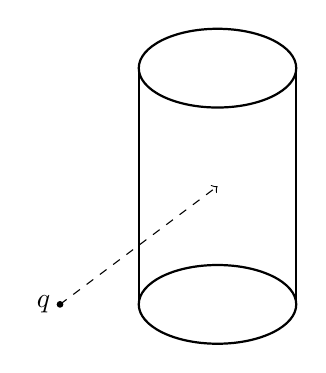
\begin{tikzpicture}
    % Cylinder
    \draw[thick] (1, 0) ellipse (1 and 0.5); % Front ellipse
    \draw[thick] (1, 3) ellipse (1 and 0.5); % Back ellipse
    \draw[thick] (0, 0) -- (0, 3); % Left side of the cylinder
    \draw[thick] (2, 0) -- (2, 3); % Right side of the cylinder

    % Dashed line and arrow for the point charge q
    \draw[dashed, ->] (-1,0) -- (1, 1.5);
    \node[left] at (-1, 0) {$q$};
    \filldraw (-1,0) circle (1pt); % Point charge q

\end{tikzpicture}
\begin{enumerate}
    \item 

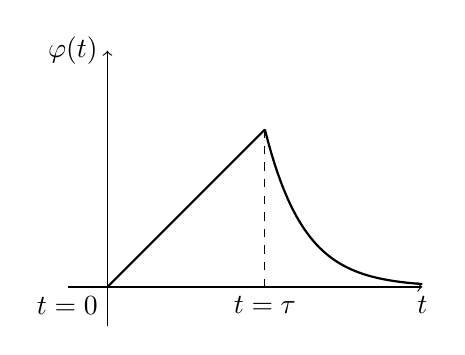
\begin{tikzpicture}
    % Axis
    \draw[->] (-0.5,0) -- (4,0) node[anchor=north] {$t$};
    \draw[->] (0,-0.5) -- (0,3) node[anchor=east] {$\varphi(t)$};
    
    % Labels
    \node at (0,0) [below left] {$t=0$};
    \node at (2,0) [below] {$t=\tau$};

    % Vertical dashed line
    \draw[dashed,-] (2,0) -- (2,2);
    \draw[thick] (0,0) -- (2,2); 


    % Curve after t = tau
    \draw[thick, domain=2:4, samples=50] plot (\x, {2*exp(-(2*(\x-2)))});

\end{tikzpicture}
\item 

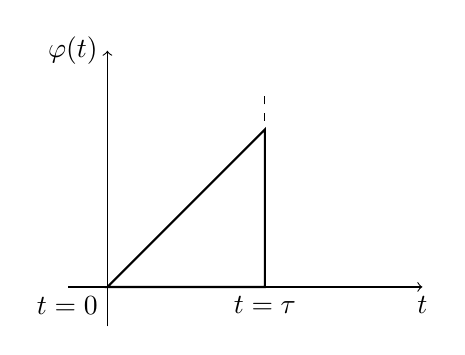
\begin{tikzpicture}
    % Axis
    \draw[->] (-0.5,0) -- (4,0) node[anchor=north] {$t$};
    \draw[->] (0,-0.5) -- (0,3) node[anchor=east] {$\varphi(t)$};
    
    % Labels
    \node at (0,0) [below left] {$t=0$};
    \node at (2,0) [below] {$t=\tau$};

    % Vertical dashed line
    \draw[dashed,-] (2,0) -- (2,2.5);

    % Triangle area
    \draw[thick] (0,0) -- (2,2) -- (2,0) -- cycle;


\end{tikzpicture}
\item 
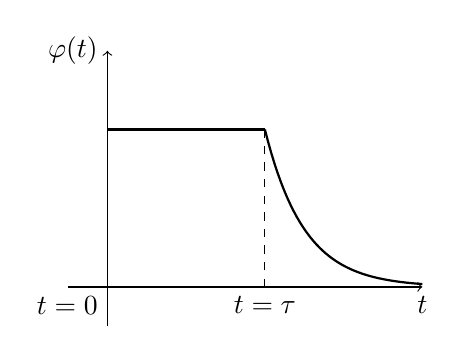
\begin{tikzpicture}
    % Axis
    \draw[->] (-0.5,0) -- (4,0) node[anchor=north] {$t$};
    \draw[->] (0,-0.5) -- (0,3) node[anchor=east] {$\varphi(t)$};
    
    % Labels
    \node at (0,0) [below left] {$t=0$};
    \node at (2,0) [below] {$t=\tau$};

    % Vertical dashed line
    \draw[dashed,-] (2,0) -- (2,2);
    \draw[thick] (0,2) -- (2,2);
    

    % Triangle area
   % \draw[thick] (0,0) -- (2,2.5) -- (2,0) -- cycle;

    % Curve after t = tau
    \draw[thick, domain=2:4, samples=50] plot (\x, {2*exp(-(2*(\x-2)))});
\end{tikzpicture}
\item 
\begin{tikzpicture}
    % Axis
    \draw[->] (-0.5,0) -- (4,0) node[anchor=north] {$t$};
    \draw[->] (0,-0.5) -- (0,3) node[anchor=east] {$\varphi(t)$};
    
    % Labels
    \node at (0,0) [below left] {$t=0$};
    \node at (2,0) [below] {$t=\tau$};

    % Vertical dashed line
    \draw[dashed,-] (2,0) -- (2,2);
    \draw[thick] (0,2) -- (2,2);
    \draw[thick] (2,2) -- (2,0);
    
    
\end{tikzpicture}

\end{enumerate}
    \item Consider a one-dimensional non-magnetic crystal with one atom per unit cell.Assume that the valence electrons $\brak{i}$ do not interact weakly with the ions. If $n$ is number of valence electrons per unit cell, then at $0K,$
    \begin{enumerate}
        \item the crystal is metallic for any value of $n$
        \item the crystal is non-metallic for any value of $n$
        \item the crystal is metallic for even value of $n$
        \item the crystal is metallic for odd value of $n$
    \end{enumerate}
    \item According to the Fermi gas model of the nucleus, the nucleons move in a spherical volume of radius $R=R_0A^{\frac{1}{3}},$where $A$ is the mass number and $R_0$ is an empirical constant with the dimensions of length.The Fermi energy of the nucleaus $E_F$ is proportional to
    \begin{enumerate}
        \item ${R_0}^2$
        \item $\frac{1}{R_0}$
        \item $\frac{1}{{R_0}^2}$
        \item $\frac{1}{{R_0}^3}$
    \end{enumerate}
    \item Consider a two dimensional crystal with $3$ atoms in the basis. The number of allowed in optical branches $\brak{n}$ and acoustic branches $\brak{m}$ due to the lattice vibrations are
    \begin{enumerate}
        \item $\brak{n,m}=\brak{2,4}$
        \item $\brak{n,m}=\brak{3,3}$
        \item $\brak{n,m}=\brak{4,2}$
        \item $\brak{n,m}=\brak{1,5}$
    \end{enumerate}
    \item The internal energy $U$ of a system is given by $U\brak{S,V}=\lambda V^{-\frac{2}{3}}S^2,$where $\lambda$ is a constant of appropriate dimensions; $V$ and $S$ denote the volume and entropy respectively. Which one of the following gives the correct equation of state of the system?
    \begin{enumerate}
        \item $\frac{PV^{\frac{1}{3}}}{T^2}=$constant
         \item $\frac{PV}{T^{\frac{1}{3}}}=$constant
        \item $\frac{PV}{v^{\frac{1}{3}}T}=$constant
        \item $\frac{PV^{\frac{2}{3}}}{T}=$constant
    \end{enumerate}
    \item The potential energy of a particle of mass $m$ is given by \\
    $U\brak{x}=a\sin\brak{k^2x-\frac{\pi}{2}},\quad a\textgreater 0,k^2\textgreater 0.$\\
    The angular frequency of small oscillations of the particle about $x=0$ is
    \begin{enumerate}
        \item $k^2\sqrt{\frac{2a}{m}}$
        \item $k^2\sqrt{\frac{a}{m}}$
        \item $k^2\sqrt{\frac{a}{2m}}$
        \item $2k^2\sqrt{\frac{a}{m}}$   
    \end{enumerate}
